\documentclass[aspectratio=169]{beamer}
\usetheme{default}
\usecolortheme{dove}

\usepackage{booktabs}
\usepackage{tikz}
\usepackage{xcolor}
\usepackage{array}

% Custom colors
\definecolor{passgreen}{RGB}{34, 139, 34}
\definecolor{warnyellow}{RGB}{255, 165, 0}
\definecolor{failred}{RGB}{178, 34, 34}

% Remove navigation symbols
\setbeamertemplate{navigation symbols}{}

% Custom checkmark and x
\newcommand{\cmark}{\textcolor{passgreen}{\checkmark}}
\newcommand{\xmark}{\textcolor{failred}{$\times$}}

\title{Referee Report --- Round 3}
\subtitle{Tennis Match Simulator: Elo Model \& Model Comparison}
\author{Referee 2}
\date{2026-02-05}

\begin{document}

% Title slide
\begin{frame}
\titlepage
\end{frame}

% Executive Summary
\begin{frame}{Minor Revisions: Elo Sound, Comparison Flawed}
\Large

\textbf{Elo model is a strong addition --- but the comparison needs fixing}

\vspace{1em}

\begin{itemize}
    \item[\xmark] Model comparison evaluates on different match samples
    \item[\xmark] MC accuracy (58.7\%) is below naive baseline ($\sim$66\%)
    \item[\xmark] K-factor averaging is non-standard in \texttt{elo\_update()}
    \item[\cmark] Elo core logic is correct and well-structured
    \item[\cmark] Rolling backtest integration prevents data leakage
    \item[\cmark] Round 2 minor concerns resolved (renv.lock generated)
\end{itemize}

\end{frame}

% Model Comparison Problem
\begin{frame}{Headline Finding Built on Different Samples}

\begin{table}
\centering
\begin{tabular}{lccc}
\toprule
& Elo Model & MC Model & Issue \\
\midrule
Accuracy & 68.2\% & 58.7\% & \\
Brier Score & 0.2056 & 0.2338 & \\
\texttt{require\_player\_data} & not set & \texttt{TRUE} & \textcolor{failred}{\textbf{Mismatch}} \\
Sample & All matches & Filtered ($\geq$20 matches) & \textcolor{failred}{\textbf{Mismatch}} \\
\bottomrule
\end{tabular}
\end{table}

\vspace{1em}

\textbf{Problem:} The Elo model sees $\sim$1,499 matches. The MC model sees $\sim$1,201 (20\% excluded for insufficient data).

\vspace{0.5em}

\textbf{The +9.6pp accuracy gap conflates model quality with sample composition.}

\vspace{0.5em}

\textbf{Fix:} Evaluate both models on the identical match set.

\end{frame}

% MC Below Baseline
\begin{frame}{MC Model Accuracy Is Below the Naive Baseline}

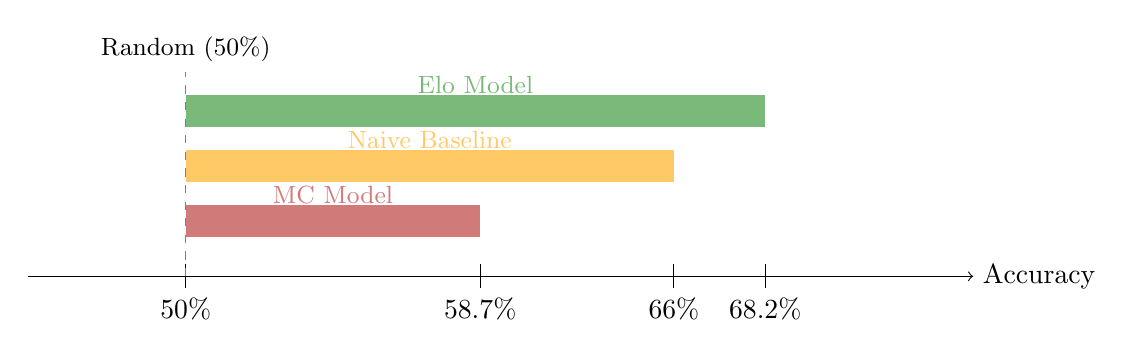
\begin{tikzpicture}
  % Axis
  \draw[->] (0,0) -- (12,0) node[right] {Accuracy};
  % Ticks and labels
  \draw (2,0.15) -- (2,-0.15) node[below] {50\%};
  \draw (5.74,0.15) -- (5.74,-0.15) node[below] {58.7\%};
  \draw (8.2,0.15) -- (8.2,-0.15) node[below] {66\%};
  \draw (9.36,0.15) -- (9.36,-0.15) node[below] {68.2\%};
  % Bars
  \fill[gray!40] (2,0.3) rectangle (2,0.8);
  \fill[failred!60] (2,0.5) rectangle (5.74,0.9) node[midway, above=0.1cm] {\small MC Model};
  \fill[warnyellow!60] (2,1.2) rectangle (8.2,1.6) node[midway, above=0.1cm] {\small Naive Baseline};
  \fill[passgreen!60] (2,1.9) rectangle (9.36,2.3) node[midway, above=0.1cm] {\small Elo Model};
  % Random line
  \draw[dashed, gray] (2,0) -- (2,2.6);
  \node[above] at (2,2.6) {\small Random (50\%)};
\end{tikzpicture}

\vspace{1em}

\textbf{Diagnosis:} The opponent adjustment formula in \texttt{01\_mc\_engine.R:62--63} likely overcorrects, pushing predictions away from true probabilities.

\vspace{0.5em}

\textbf{Test:} Run MC with \texttt{use\_adjustment = FALSE} to isolate the effect.

\end{frame}

% K-Factor Bug
\begin{frame}{K-Factor Averaging Slows Convergence for New Players}

\begin{columns}
\begin{column}{0.5\textwidth}
\textbf{Current (non-standard):}
\begin{itemize}
    \item \texttt{k\_avg = (48 + 32) / 2 = 40}
    \item Winner gains 20 points
    \item Loser loses 20 points
\end{itemize}

\vspace{0.5em}
\textcolor{failred}{Provisional player learns 17\% slower}
\end{column}

\begin{column}{0.5\textwidth}
\textbf{Standard Elo:}
\begin{itemize}
    \item Winner uses own K=48
    \item Loser uses own K=32
    \item Winner gains 24, loser loses 16
\end{itemize}

\vspace{0.5em}
\textcolor{passgreen}{Each player's K reflects their uncertainty}
\end{column}
\end{columns}

\vspace{1.5em}

\textbf{Impact:} Moderate. Affects early-career ratings most. Both approaches are zero-sum in aggregate but per-player K is the standard for a reason: new players should move faster.

\end{frame}

% Elo Implementation Review
\begin{frame}{Elo Core Implementation Is Clean}

\begin{table}
\centering
\begin{tabular}{lcc}
\toprule
Component & Status & Notes \\
\midrule
\texttt{elo\_expected\_prob()} & \cmark & Standard formula \\
\texttt{elo\_update()} & \textcolor{warnyellow}{$\circ$} & K-factor averaging (see previous) \\
\texttt{calculate\_all\_elo()} & \cmark & Correct chronological processing \\
\texttt{get\_player\_elo()} & \cmark & Linear surface blend is reasonable \\
\texttt{predict\_match\_elo()} & \cmark & Clean interface \\
Surface-specific tracking & \cmark & Hard, Clay, Grass \\
Rolling backtest rebuild & \cmark & No data leakage \\
Unit tests & \textcolor{warnyellow}{$\circ$} & Present but limited coverage \\
\bottomrule
\end{tabular}
\end{table}

\vspace{0.5em}

\textbf{Minor:} Surface Elo starts at 1500 instead of player's overall Elo. Mitigated by blending at prediction time.

\end{frame}

% Replication Readiness
\begin{frame}{Replication Readiness: 8/10 (up from 7/10)}


\begin{tikzpicture}
  % Progress bar
  \fill[passgreen!70] (0,0) rectangle (8,0.5);
  \fill[gray!30] (8,0) rectangle (10,0.5);
  \node at (5,0.25) {\textbf{\textcolor{white}{8/10}}};
\end{tikzpicture}

\vspace{1em}

\begin{columns}
\begin{column}{0.5\textwidth}
\textcolor{passgreen}{\cmark} Folder structure \\
\textcolor{passgreen}{\cmark} Relative paths \\
\textcolor{passgreen}{\cmark} Variable naming \\
\textcolor{passgreen}{\cmark} Script naming \\
\textcolor{passgreen}{\cmark} Master script \\
\textcolor{passgreen}{\cmark} README \\
\textcolor{passgreen}{\cmark} Random seeds \\
\textcolor{passgreen}{\cmark} renv.lock \textbf{(NEW)}
\end{column}

\begin{column}{0.5\textwidth}
\textcolor{warnyellow}{$\circ$} Compare script not in pipeline \\
\textcolor{warnyellow}{$\circ$} No cross-language Elo replication \\
\textcolor{gray}{---} Automated figures (low priority) \\
\textcolor{gray}{---} In-text stats automation (low priority)
\end{column}
\end{columns}

\end{frame}

% Questions for Authors
\begin{frame}{Questions for Authors}

\begin{enumerate}
    \item What is MC accuracy with \texttt{use\_adjustment = FALSE}?
    \begin{itemize}
        \item If $\sim$65\%, the adjustment formula is the problem, not point-level simulation
    \end{itemize}

    \vspace{0.5em}

    \item What is Elo accuracy on the \textbf{same sample} as the MC model?
    \begin{itemize}
        \item Restrict to matches where both players have $\geq$20 real matches
    \end{itemize}

    \vspace{0.5em}

    \item Was K=32 chosen by convention or sensitivity analysis?
    \begin{itemize}
        \item Some tennis Elo implementations use K=20--24
    \end{itemize}

    \vspace{0.5em}

    \item Has the hybrid model been explored?
    \begin{itemize}
        \item Elo for win probability, MC for score-level predictions
    \end{itemize}
\end{enumerate}

\end{frame}

% Recommendations
\begin{frame}{Recommendations (Priority Order)}

\begin{enumerate}
    \item \textbf{Fix the model comparison} --- evaluate both models on the identical match set

    \vspace{0.3em}

    \item \textbf{Diagnose MC underperformance} --- test without opponent adjustment

    \vspace{0.3em}

    \item \textbf{Fix K-factor averaging} --- use per-player K-factors in \texttt{elo\_update()}

    \vspace{0.3em}

    \item \textbf{Extend unit tests} --- add unequal K-factor test, integration tests

    \vspace{0.3em}

    \item \textit{Optional:} K-factor sensitivity analysis (K=20, 24, 32, 40)

    \vspace{0.3em}

    \item \textit{Optional:} Initialize surface Elo from overall Elo
\end{enumerate}

\end{frame}

% Final Verdict
\begin{frame}{Verdict: Minor Revisions}

\begin{center}
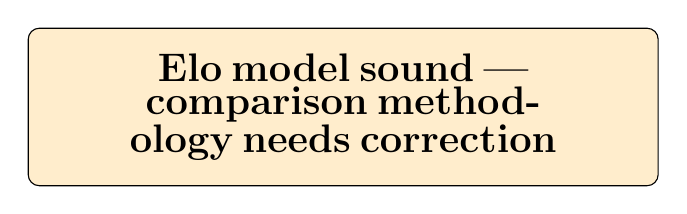
\begin{tikzpicture}
    \node[draw, rounded corners, fill=warnyellow!20, minimum width=8cm, minimum height=2cm, text width=7.5cm, align=center] {
        \Large \textbf{Elo model sound --- comparison methodology needs correction}
    };
\end{tikzpicture}
\end{center}

\vspace{1em}

\textbf{Before the +9.6pp headline can stand:}

\begin{enumerate}
    \item Run both models on the same matches
    \item Diagnose why MC is below the naive baseline
    \item Fix K-factor averaging bug
\end{enumerate}

\vspace{1em}

\textbf{No re-review required} if sample alignment and K-factor fix are straightforward.

\end{frame}

\end{document}
